\subsection{Sparse-Sparse Matrix Multiply (SpGEMM)}

\begin{figure}[b]
    \begin{minipage}[t]{0.32\linewidth}
      \vspace{0pt}
    \begin{minted}{julia}
    @finch begin
      C .= 0
      for j=_
        for i=_
          for k=_
            C[i, j] += AT[k, i] * B[k, j]
          end
        end
      end
      return C
    end
    \end{minted}
    \end{minipage}%
    \begin{minipage}[t]{0.33\linewidth}
      \vspace{0pt}
    \begin{minted}{julia}
    w = Tensor(SparseByteMap(Element(0)))
    @finch begin
      C .= 0
      for j=_
        w .= 0
        for k=_
          for i=_
            w[i] += A[i, k] * B[k, j]
          end
        end
        for i=_
          C[i, j] = w[i]
        end
      end
    end
    \end{minted}
    \end{minipage}%
    \begin{minipage}[t]{0.35\linewidth}
      \vspace{0pt}
    \begin{minted}{julia}
    w = Tensor(SparseHash(SparseHash(Element(0))))
    @finch begin
      w .= 0
      for k=_
        for j=_
          for i=_
            w[i, j] += A[i, k] * BT[j, k]
          end
        end
      end
      C .= 0
      for j=_, i=_
        C[i, j] = w[i, j]
      end
    end
    \end{minted}
    \end{minipage}
    \caption{Inner Products, Gustavsons, and Outer Products matrix multiply in Finch}\label{fig:spgemm_listing}
\end{figure}


\begin{figure}[b]
	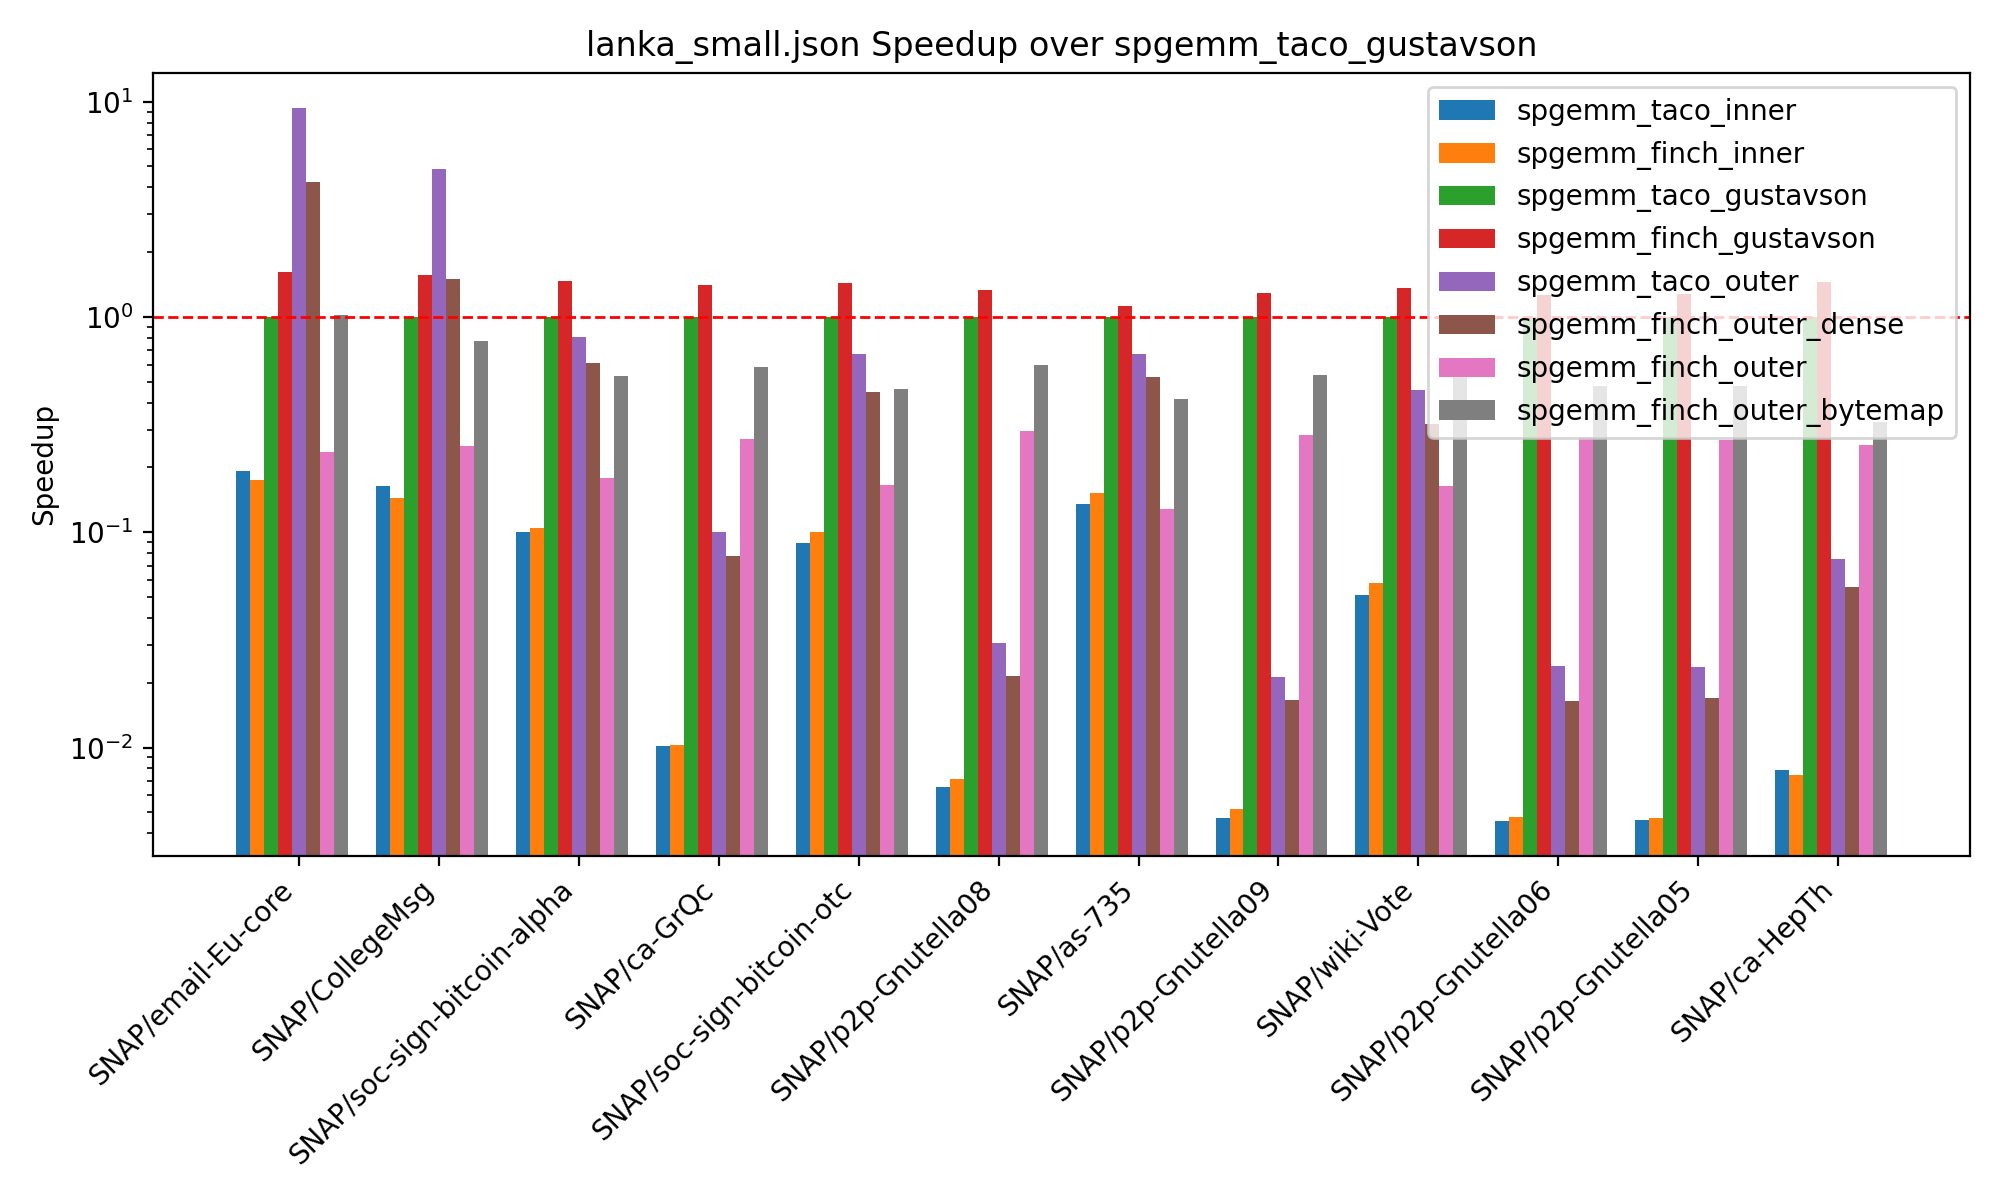
\includegraphics[width=0.5\linewidth]{spgemm_small_speedup_log_scale.png}%
	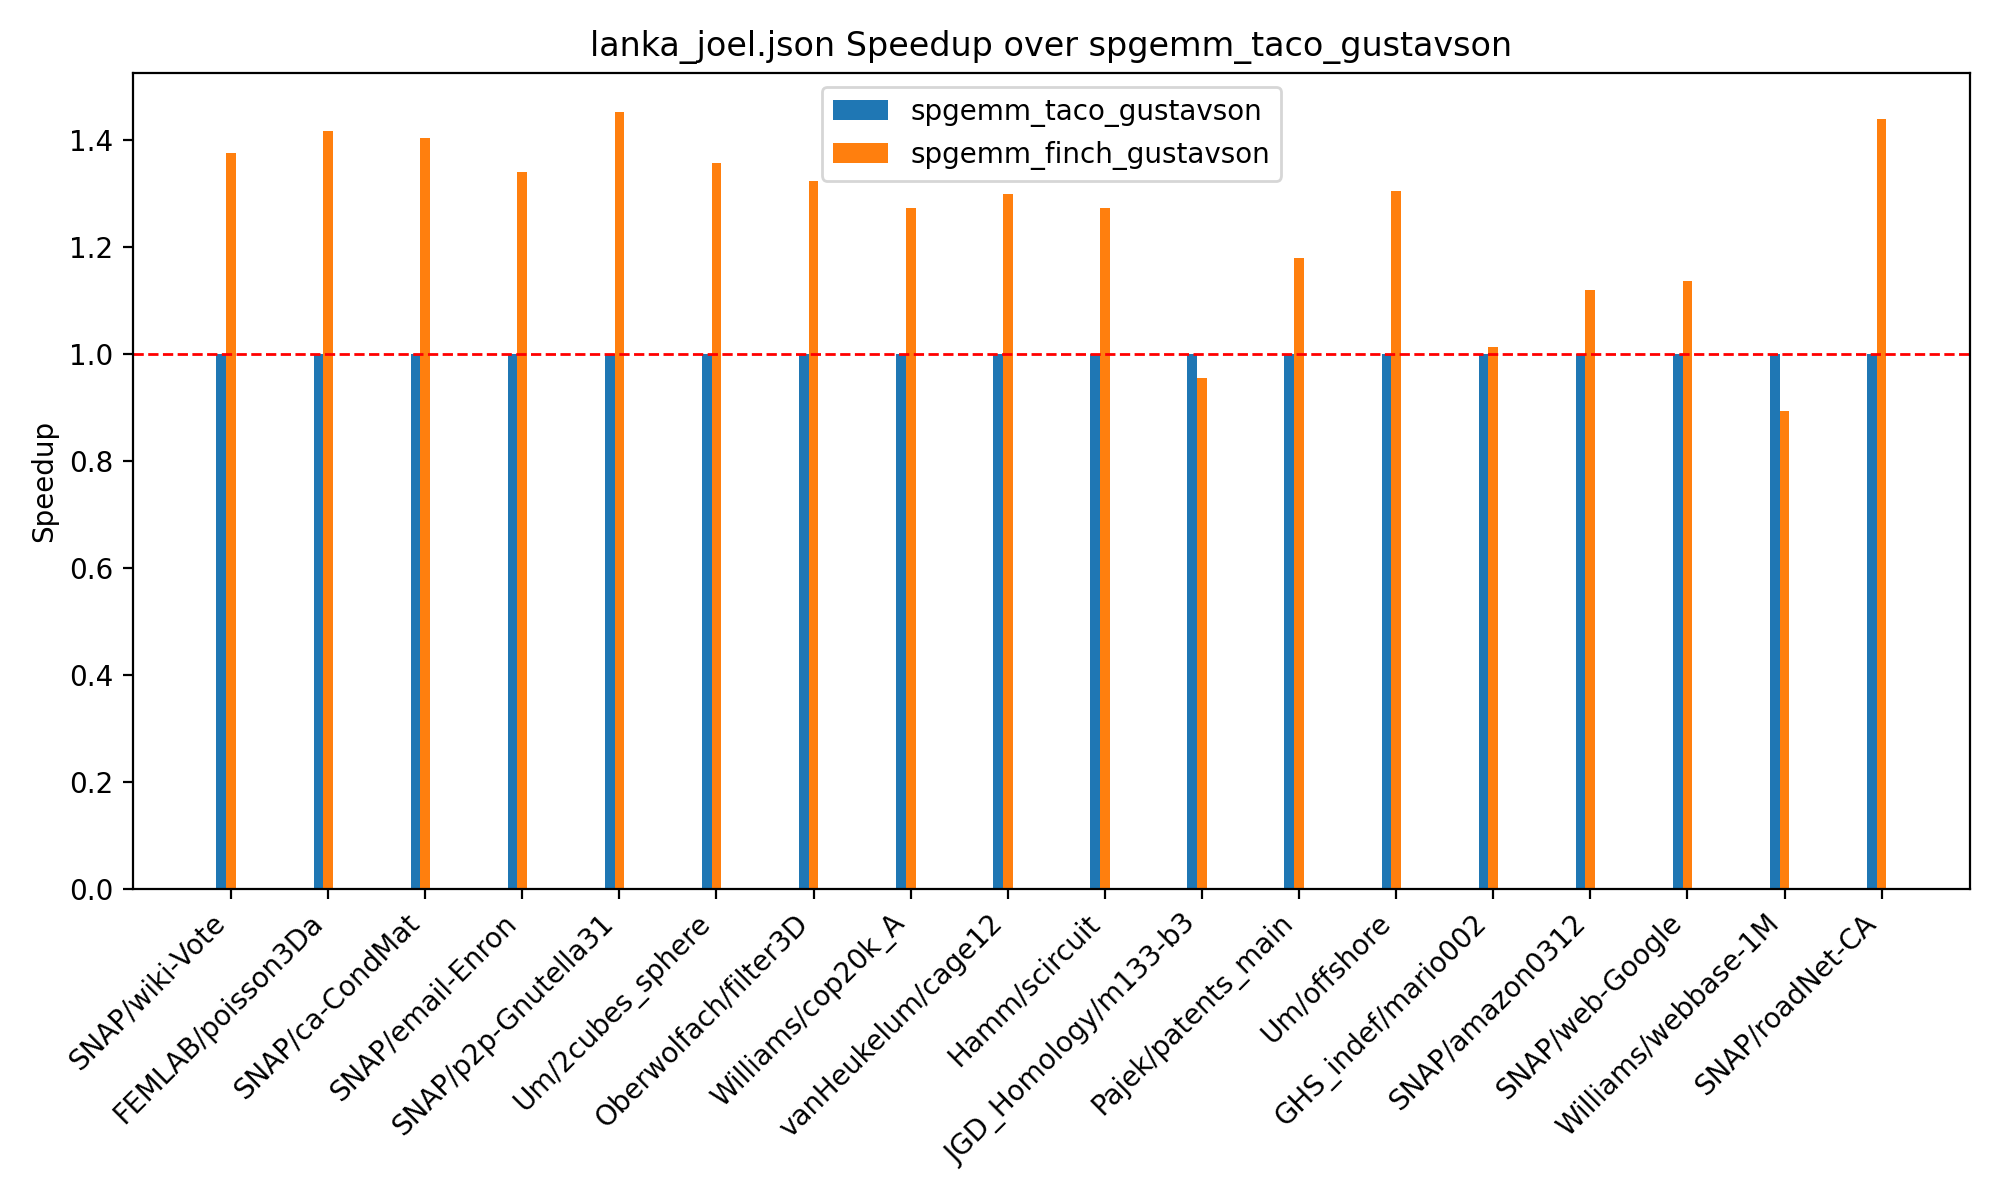
\includegraphics[width=0.5\linewidth]{spgemm_joel_speedup.png}
    \vspace{-8pt}
    \caption{A comparison of several matrix multiply algorithms between
    Finch and Taco. On left, we use smaller matrices, ordered from small to big
    dimension. Note that inner-products necessarily requires $O(MN)$ work and
    TACO's outer-products format is dense. Finch can use a sparse outer products
    format and thus has an asymptotic advantage that becomes evident as the
    output dimensions grow. On right, we use only gustavson's algorithm and
    compare on larger matrices.}
    \label{fig:spgemm}
    \vspace{-12pt}
\end{figure}


%Sparse Matrix-Matrix Multiplication (SpGEMM) is a fundamental operation in scientific computing and data analytics. 
We compute the $M \times N$ sparse matrix $C$ as the product of $M \times K$ and $K \times N$ sparse matrices $A$ and $B$.
%
There are three main approaches to SpGEMM \cite[Section 2.2]{zhang2021gamma}.
%
The inner-products algorithm takes dot products of corresponding rows and columns, while the outer-products algorithm sums the outer products of corresponding columns and rows.
%
Gustavson's algorithm sums the rows of $B$ scaled by the corresponding nonzero columns in each row of $A$.
%
Inner-products is known to be asymptotically less efficient than the others, as we must do a merge operation to compute each of the $O(MN)$ entries in the output \cite{ahrens2022autoscheduling}.
%
We will show that our ability to implement these latter methods exceeds that of TACO, translating to asymptotic benefits. 
% 

Figure~\ref{fig:spgemm_listing} implements all three approaches in Finch, and Figure~\ref{fig:spgemm} compares the performance of Finch to TACO.
%
Note that these algorithms mainly differ in their loop order, but that different data structures can be used to support the various access patterns induced.
%
In our Finch implementation of outer products, we use a sparse hash table, as it is fully-sparse and randomly accessible.
%
Since, TACO does not support multidimensional sparse workspaces, its outer products uses a dense intermediate, which leads to an asymptotic slow down shown in Figure~\ref{fig:spgemm}.
%
Similarly, although a sparse bytemap has a dense memory footprint, we use it in our Finch implementation of Gustavson's for the smaller $O(N)$ intermediate.
%
We note that the bytemap format in TACO's Gustavson's implementation is hard-wired, whereas Finch's programming model allows us to write algorithms with explicit temporaries and transpositions.
%
Without such hard wiring, TACO would have to use a dense intermediate to support random writes, which TACO would then propagate to the output, turning it dense and leading to the same asymptotic results as in the case of outer products. 
%
As depicted in Figure~\ref{fig:spgemm}, Finch achieves comparable performance with TACO on smaller matrices when we use the same datastructures, and significant improvements when we use better datastructures. 
%
Finch outperforms TACO on larger matrices, with an average speedup of 1.25. %arith-mean

%\changwan{(self)may remove this number for consistency with other exps. finch\_outer\_bytemap not explained.}
